\subsection*{Problema 12}

\textbf{Enunciado:}
Calcular la integral indefinida:
\begin{equation*}
  \int \frac{x}{\sqrt{1 + x - x^2}} \, dx
\end{equation*}

\textbf{Solución:}
Siguiendo las indicaciones, reescribimos el numerador para que aparezca la derivada del argumento dentro de la raíz. 
Sea $u = 1 + x - x^2$, su derivada es $u' = 1 - 2x$. 
Modificamos el numerador del integrando:
\begin{align*}
  x &= -\frac{1}{2}(-2x) \\
  &= -\frac{1}{2}(1 - 2x - 1) \\
  &= -\frac{1}{2}(1 - 2x) + \frac{1}{2}
\end{align*}

Sustituimos esto en la integral original y separamos en dos partes:
\begin{align*}
  I &= \int \dfrac{-\frac{1}{2}(1 - 2x) + \frac{1}{2}}{\sqrt{1 + x - x^2}} \, dx \\
  &= -\frac{1}{2} \int \dfrac{1 - 2x}{\sqrt{1 + x - x^2}} \, dx \\
  &\quad + \frac{1}{2} \int \dfrac{1}{\sqrt{1 + x - x^2}} \, dx
\end{align*}

Para la primera integral, aplicamos sustitución directa con $u = 1 + x - x^2$ y $du = (1 - 2x) \, dx$:
\begin{align*}
  I_1 &= -\frac{1}{2} \int u^{-1/2} \, du \\
  &= -\frac{1}{2} \left( 2u^{1/2} \right) \\
  &= -\sqrt{1 + x - x^2}
\end{align*}

Para la segunda integral, completamos el cuadrado en el trinomio del denominador:
\begin{align*}
  1 + x - x^2 &= 1 - \left( x^2 - x \right) \\
  &= 1 - \left( x^2 - x + \frac{1}{4} - \frac{1}{4} \right) \\
  &= \frac{5}{4} - \left( x - \frac{1}{2} \right)^2
\end{align*}

Sustituimos esto en la segunda integral:
\begin{align*}
  I_2 &= \frac{1}{2} \int \dfrac{dx}{\sqrt{\left(\frac{\sqrt{5}}{2}\right)^2 - \left(x - \frac{1}{2}\right)^2}}
\end{align*}

Esta es una integral directa del tipo arcoseno:
\begin{align*}
  I_2 &= \frac{1}{2} \arcsin\left( \dfrac{x - \frac{1}{2}}{\frac{\sqrt{5}}{2}} \right) \\
  &= \frac{1}{2} \arcsin\left( \dfrac{2x - 1}{\sqrt{5}} \right)
\end{align*}

Finalmente, unimos ambos resultados y agregamos la constante de integración $C$:
\begin{align*}
  I &= -\sqrt{1 + x - x^2} \\
  &\quad + \frac{1}{2} \arcsin\left( \dfrac{2x - 1}{\sqrt{5}} \right) + C
\end{align*}

\begin{figure}[H]
	\centering
	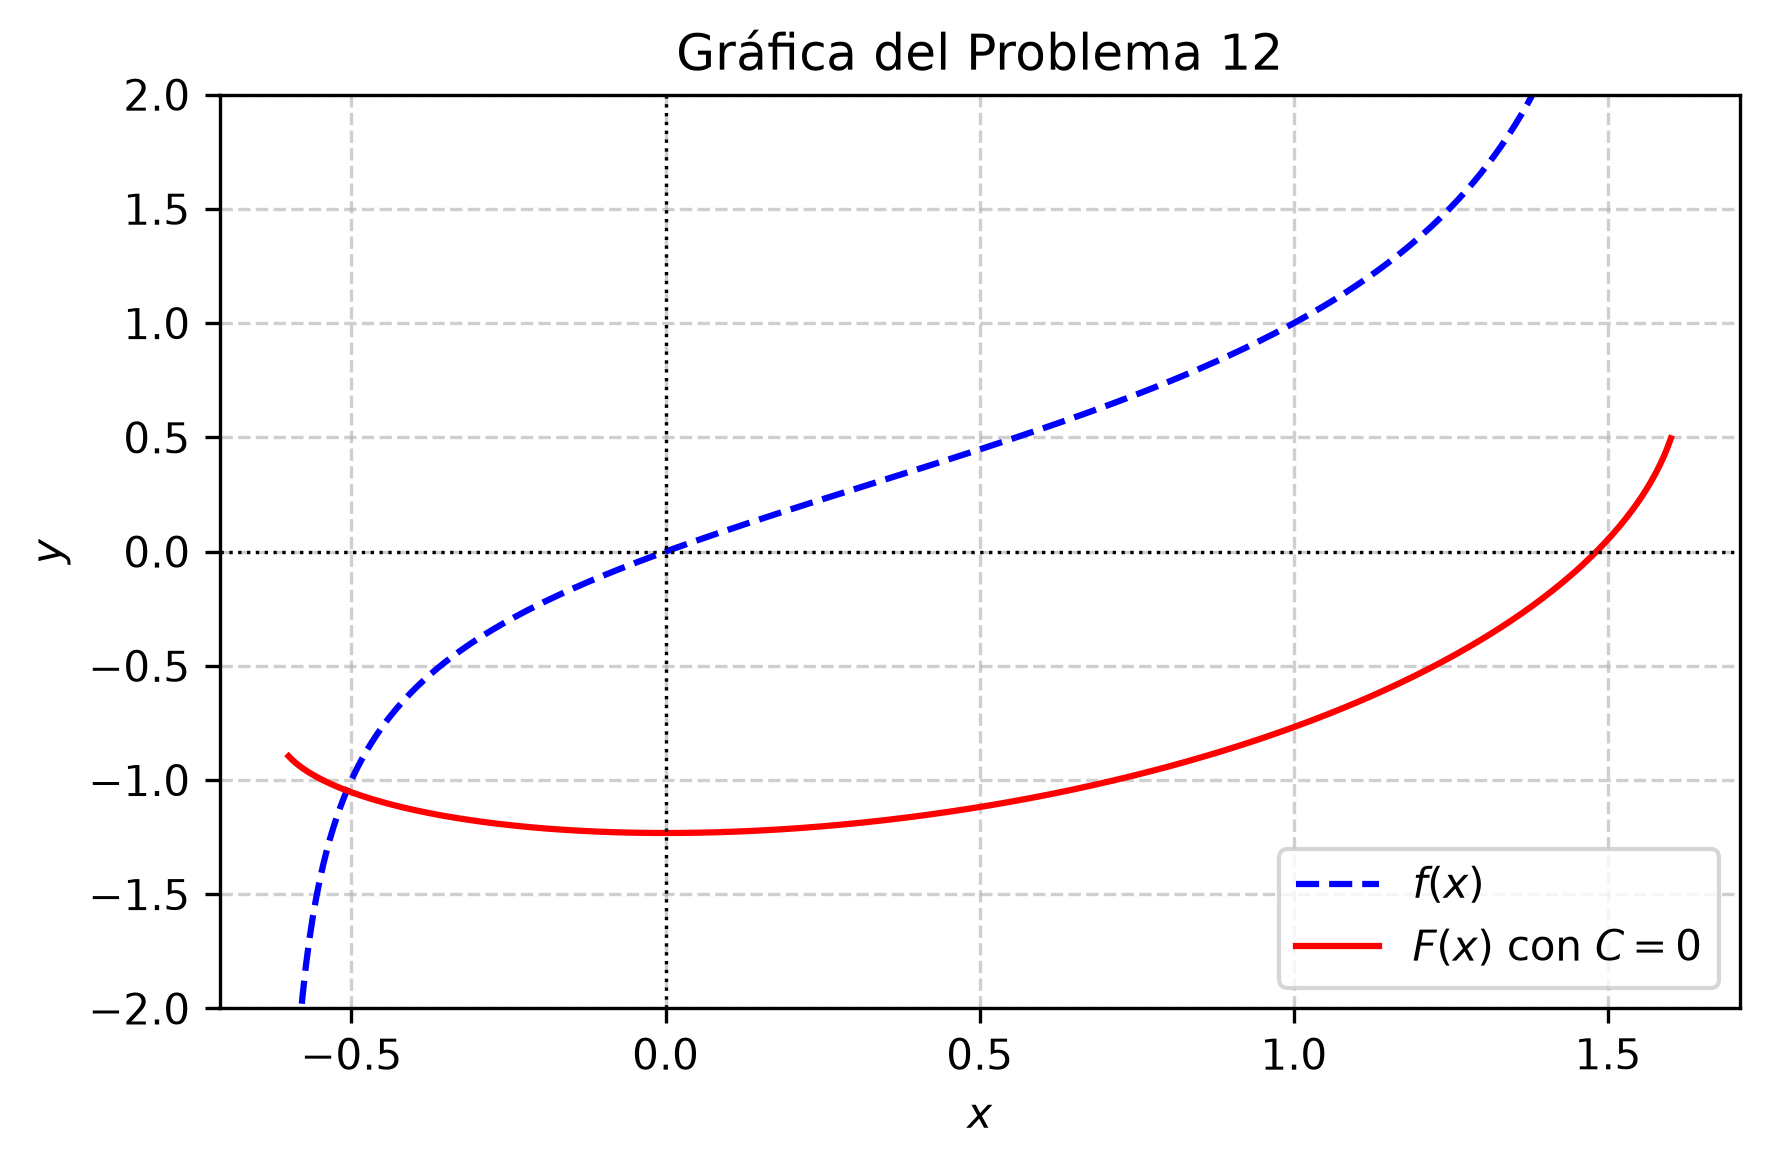
\includegraphics[width=\columnwidth]{semana_05/graficas/SEM05_P12_grafica.png}
	\caption{Representación gráfica de $f(x)$ y su antiderivada $F(x)$ evaluada para la constante de integración $C = 0$ (Problema 12).}
	\label{fig:problema12}
\end{figure}
